\documentclass{article}
\usepackage{geometry}
\usepackage{graphicx}
\usepackage{titlesec}
\usepackage{fancyhdr}
\usepackage{threeparttable} % Add this to your preamble
\usepackage{rotating} % Add this to your preamble
\usepackage{tikz}
\usepackage{float} % Add this to your preamble
\usepackage{graphicx} % Ensure this is in your preamble


\usetikzlibrary{shapes.geometric, arrows}

\geometry{a4paper, margin=1in}

% Custom section title
\titleformat{\section}
  {\normalfont\Large\bfseries\centering}{\thesection}{1em}{}

% Header
\pagestyle{fancy}
\fancyhf{}
\fancyhead[L]{\textit{Epilepsia, 51(7):1177--1184, 2010}\\
doi: 10.1111/j.1528-1167.2009.02426.x}

\tikzstyle{startstop} = [rectangle, rounded corners, minimum width=3cm, minimum height=1cm, text centered, draw=black, fill=gray!30]
\tikzstyle{process} = [rectangle, minimum width=3cm, minimum height=1cm, text centered, draw=black, fill=gray!10]
\tikzstyle{arrow} = [thick,->,>=stealth]

\begin{document}

\setlength{\headheight}{23.10004pt}
% Title Box
\begin{center}
  \fbox{\parbox{\textwidth}{
    \centering
    \textbf{\large FULL-LENGTH ORIGINAL RESEARCH}
  }}
\end{center}

% Main Title
\begin{center}
  \textbf{\LARGE Alcohol consumption, unprovoked seizures, and epilepsy:}\\
  \textbf{\LARGE A systematic review and meta-analysis}
\end{center}

% Authors
\begin{center}
  \textbf{*Andriy V. Samokhvalov, *Hyacinth Irving, *Satya Mohapatra, and *†‡Jürgen Rehm}
\end{center}

% Affiliations
\begin{center}
  \textit{*Public Health and Regulatory Policy, Centre for Addiction and Mental Health, Toronto, Ontario, Canada;}\\
  \textit{†Dalla Lana School of Public Health, University of Toronto, Toronto, Canada; and ‡Epidemiological Research Unit,}\\
  \textit{Klinische Psychologie \& Psychotherapie, Technische Universität, Dresden, Germany}
\end{center}

% Summary Section
\section*{Summary}
\textbf{Purpose:} The purpose of this research was to analyze and quantify the association between alcohol consumption and epilepsy as an independent disease, in part operationalized by the occurrence of unprovoked seizures, as well as to examine causality.\\
\textbf{Methods:} Systematic review, meta-analysis.\\
\textbf{Results:} A strong and consistent association between alcohol consumption and epilepsy/unprovoked seizures was found with an overall relative risk (RR) of 2.19 [95\% confidence interval (CI) 1.83–2.63]. There was a dose–response relationship between the amount of alcohol consumed daily and the probability of the onset of epilepsy. Individuals consuming an average of four, six, and eight drinks daily had RRs of 1.81 (95\% CI 1.59–2.07), 2.44 (95\% CI 2.00–2.97), and 3.27 (95\% CI 2.52–4.26), respectively, compared to nondrinkers. Several pathogenic mechanisms for the development of epilepsy in alcohol users were identified. Most of the relevant studies found that a high percentage of alcohol users with epilepsy would qualify for the criteria of alcohol dependence. Data were inconclusive regarding a threshold for the effect of alcohol, but most studies suggest that the effect may only hold for heavy drinking (four and more drinks daily).\\
\textbf{Discussion:} The relationship between alcohol consumption and epilepsy and unprovoked seizures was quantified and several pathogenic mechanisms were suggested, although none of them has been proven to be the unique causative pathway for epilepsy. Certain limitations underlying this study require further research to clarify the outstanding statistical issues and pathogenesis of epilepsy in heavy drinkers.\\
\textbf{KEY WORDS:} Alcohol, Heavy drinking, Alcohol dependence, Epilepsy, Unprovoked seizures.

% Add this text to the document
\section*{Introduction}
Epilepsy is one of the most common neurologic conditions, with an annual incidence in industrialized countries of 40–70 per 100,000 people. The prevalence of recurrent unprovoked seizures ranges from 370 per 100,000 in Iceland to 800 per 100,000 in Poland and the Faroe Islands (Jallon, 2002). Lifetime prevalence rates of the different types of seizures are much higher than prevalence rates of active epilepsy. It has been estimated that up to 5\% of the population will experience nonfebrile seizures at some point in their lives (Bell \& Sander, 2001). In 2000, epilepsy contributed more than 7 million disability adjusted life-years DALYs, 0.5\% of the global burden of disease (Leonardi \& Ustun, 2002). In addition to its relatively high prevalence, epilepsy is a highly stigmatized disease (Jacoby, 2002; Fernandes et al., 2004).

Alcohol consumption, one of five most important risk factors for the global burden of disease and disability (Ezzati et al., 2002; Rehm et al., 2003), has been shown to be associated with epilepsy (English et al., 1995). Numerous studies have examined the complex relationship between alcohol consumption and epilepsy, with the main focus on alcohol-induced seizures due to withdrawal (Alldredge \& Lowenstein, 1993; Hillbom et al., 2003). However, few studies have examined the onset of epilepsy as an independent disease as well as the occurrence of unprovoked seizures among alcohol users. Both factors may be crucial in determining the causal role of alcohol as an independent risk factor for epilepsy. This is in line with the possibility that many disease events labeled as epilepsy are alcohol-withdrawal seizures rather than unprovoked seizures. This study aimed to analyze and quantify the association and dose–response relationship between alcohol consumption and epilepsy, with the particular focus on examining potential mechanisms.


\section*{Methods}
\textbf{Definition of outcome}


For this study, we used the definition of epilepsy derived from the International League Against Epilepsy (ILAE) and the International Bureau for Epilepsy (IBE). According to the ILAE and the IBE, epilepsy is a disorder of the brain that is characterized by an enduring predisposition to generate epileptic seizures. This definition of epilepsy requires the occurrence of at least one epileptic seizure (Fisher et al., 2005). In line with this definition, we included studies in the meta-analysis that reported unprovoked seizures or epilepsy as their outcomes.

\textbf{Systematic search of the literature and extraction of data}


A computer-based systematic literature search was completed using Ovid MEDLINE, EMBASE, Web of Science, CINAHL, PsychINFO, ETOH, and Google Scholar. The period of search was from January 1960 to September 2008 (performed in October 2008), had no language restrictions, and used all combinations of the key words: alcohol* (truncated), alcohol, alcohol consumption, alcohol intake, drinking, alcoholism, alcohol abuse, alcohol misuse, epilep* (truncated), epilepsy, epileptic, seizures. In addition, major epidemiologic journals and reference lists of relevant articles were reviewed manually.

The inclusion criteria for reviewed articles were:
\begin{enumerate}
  \item A case–control or cohort design.
  \item The inclusion of hazard ratios (HRs), relative risks (RRs) or odds ratios (ORs), with 95% confidence intervals (CIs) (or information allowing for their calculation).
  \item The endpoint being epilepsy morbidity (as defined by physician) or unprovoked seizures.
  \item Three or more categories of alcohol consumption reported (for dose–response analysis).
\end{enumerate}

Exclusion criteria were:
\begin{enumerate}
  \item A cross-sectional design or other designs without any control.
  \item Data that did not allow for a calculation of risk for relevant exposure variables.
  \item Studies on primarily alcohol-induced seizures as well as any seizures provoked by other factors (strokes, inflammation, etc.).
\end{enumerate}

If multiple published reports based on the same study data were found, the study with the most comprehensive data on alcohol consumption was included in the meta-analysis. The literature search resulted in 1,360 articles, 18 of which quantified the association between alcohol consumption and epilepsy. If the study presented information separately for different cohorts of patients or outcome categories, the data were extracted into separate datasets. In the studies by Leone et al. (1997) and Ng et al. (1988), information was presented separately for male and female subjects and was extracted as datasets (a) and (b) correspondingly for each study.



The study by Leone et al. (2002) provided data sepa-
rately for two distinctive cohorts of patients. We also cre-
ated two datasets for this study: one for subjects with
unprovoked symptomatic seizures (dataset a) and the other
for subjects with cryptogenic/idiopathic seizures (dataset b).
In total, six studies, comprising nine independent datasets,
met the inclusion criteria (see Table 1). Detailed informa-
tion on selection of studies is presented in Fig. 1.
For statistical purposes, alcohol consumption was con-
verted to average grams of pure alcohol per day. A midpoint
was calculated when alcohol consumption was given in
ranges. In cases of open-ended categories, 75% of the width
of the previous range category was added to the lower bound
of such categories.
\textbf{Statistical meta-analysis}
We first examined the association between alcohol con-
sumption (any drinking vs. no drinking) and the risk of epi-
lepsy. To do this, we pooled the RRs (weighted by the
inverse of their variance) for all drinking categories from
each study to derive a single RR for each study. The natural
logarithms of the RRs were calculated and a random-effects
model was used to derive a summary RR comparing any
drinking versus no drinking (the reference category) for all
studies combined (DerSimonian \& Laird, 1986).
We also completed another categorical meta-analysis
comparing the RR of epilepsy for daily alcohol consumption
below 50 g compared with nondrinkers to identify a potential
threshold relationship (i.e., epilepsy is only linked to heavy
drinking). We pooled the RRs (weighted by the inverse of
their variance) for all drinking categories below 50 g from
each study to derive a single RR for each study to compare to
no drinking using the same methodology as described earlier
for the alcohol yes/no dichotomy. Both categorical analyses
were completed using the metan command in STATA 10.1
(Stata Corporation, College Station, TX, U.S.A.).
To assess the dose–response relationship between alcohol
consumption and the risk of epilepsy we used the method
proposed by Greenland et al. (Greenland \& Longnecker,
1992; Orsini \& Greenland, 2006) to back-calculate and pool
the risk estimates. Only studies that provided the number of
cases and controls, and RRs with variance estimates for
three or more quantitative exposure categories of alcohol
consumption were included. For the regression, we used the
midpoints described previously. To derive the dose–
response curve, we fitted a family of first- and second-
degree fractional polynomial models (Royston \& Sauerbrei,
2008). All models were fitted using (DerSimonian \& Laird,
1986) random-effects models. The best fitting model was
selected based on a closed-test comparison between frac-
tional polynomial models (Royston \& Sauerbrei, 2008), and
overall model fit was assessed using the Cochrane Q statis-
tic (Higgins \& Thompson, 2002; Higgins et al., 2003).
These analyses were completed using the GLST command
in STATA 10.1


% ... existing code ...
\small


% ... existing code ...
\begin{sidewaystable}[h]
    \centering
    \small % Reduce font size
    
    \caption{Characteristics of the included studies}
    \begin{threeparttable}
    \begin{tabular}{|p{2.5cm}|p{3cm}|p{1.5cm}|p{2cm}|p{1cm}|p{1cm}|p{7.5cm}|p{2cm}|}
    \hline
    \textbf{Author(s)} & \textbf{Place and time of study} & \textbf{Gender} & \textbf{Study design} & \textbf{Cases} & \textbf{Controls} & \textbf{Exposure categories} & \textbf{Outcome} \\ \hline
    Zeng et al. (2003) & China, 2000 & Both & Case--control & 81 & 81 & Alcohol intake not specified & Primary epilepsy \\ \hline
    Leone et al. (2002; a)\textsuperscript{a} & Italy, January 1995--October 1998 & Both & Case--control & 33 & 59 & Current abstainers (drank no more than once a year) and occasional drinkers (drank at least once a year, but less than once a month); Current drinkers ranged by average daily alcohol intake (>50 and $\leq$ 50 g/day) & Unprovoked symptomatic seizures \\ \hline
    Leone et al. (2002; b)\textsuperscript{a} & Italy, January 1995--October 1998 & Both & Case--control & 139 & 220 & Current abstainers (drank no more than once a year) and occasional drinkers (drank at least once a year, but less than once a month); Current drinkers ranged by average daily alcohol intake (>50 and $\leq$ 50 g/day) & Idiopathic/Cryptogenic seizures \\ \hline
    Leone et al. (1997; a)\textsuperscript{a} & Italy, February 1992--October 1993 & Males & Case--control & 152 & 296 & Current abstainers (drank no more than once a year) and occasional drinkers (drank at least once a year, but less than once a month); Current drinkers ranged by average daily alcohol intake (1--25; 26--50; 51--100; 101--200; 200+ g/day) & Generalized tonic--clonic seizures \\ \hline
    Leone et al. (1997; b)\textsuperscript{a} & Italy, February 1992--October 1993 & Females & Case--control & 77 & 151 & Current abstainers (drank no more than once a year) and occasional drinkers (drank at least once a year, but less than once a month); Current drinkers ranged by average daily alcohol intake (1--25; 26--50; 51--100; 101--200; 200+ g/day) & Generalized tonic--clonic seizures \\ \hline
    Leone et al. (1994) & Italy, January 1990--March 1991 & Both & Case--control & 81 & 169 & Ex-drinkers (used to drink at least once a month and had abstained for at least 1 year); Drinkers ranged by average daily alcohol intake (>50 and $\leq$ 50 g/day) & Unprovoked seizures \\ \hline
    Ng et al. (1988; a)\textsuperscript{a} & U.S.A., December 1981--February 1984 & Males & Case--control & 145 & 128 & Abstainers (both current and lifetime); Drinkers ranged by average daily alcohol intake (1--50; 51--100; 101--200; 201--300; 300+ g/day) & Unprovoked seizures \\ \hline
    Ng et al. (1988; b)\textsuperscript{a} & U.S.A., December 1981--February 1984 & Females & Case--control & 71 & 139 & Abstainers (both current and lifetime); Drinkers ranged by average daily alcohol intake (1--50; 51--100; 101--200; 201--300; 300+ g/day) & Unprovoked seizures \\ \hline
    Ogunniyi et al. (1987) & Nigeria, September 1983--December 1984 & Both & Case--control & 155 & 155 & Alcohol intake not specified & Epilepsy \\ \hline
    \end{tabular}
    \begin{tablenotes}
    \item \textsuperscript{a}Several studies had two sets of data, named correspondingly a and b. For statistical purposes the datasets taken from the same study were used separately.
    \end{tablenotes}
    \end{threeparttable}
\end{sidewaystable}

    \normalsize



    \begin{figure}[h]
        \centering
        \caption{Study selection process. Epilepsia ILAE}
        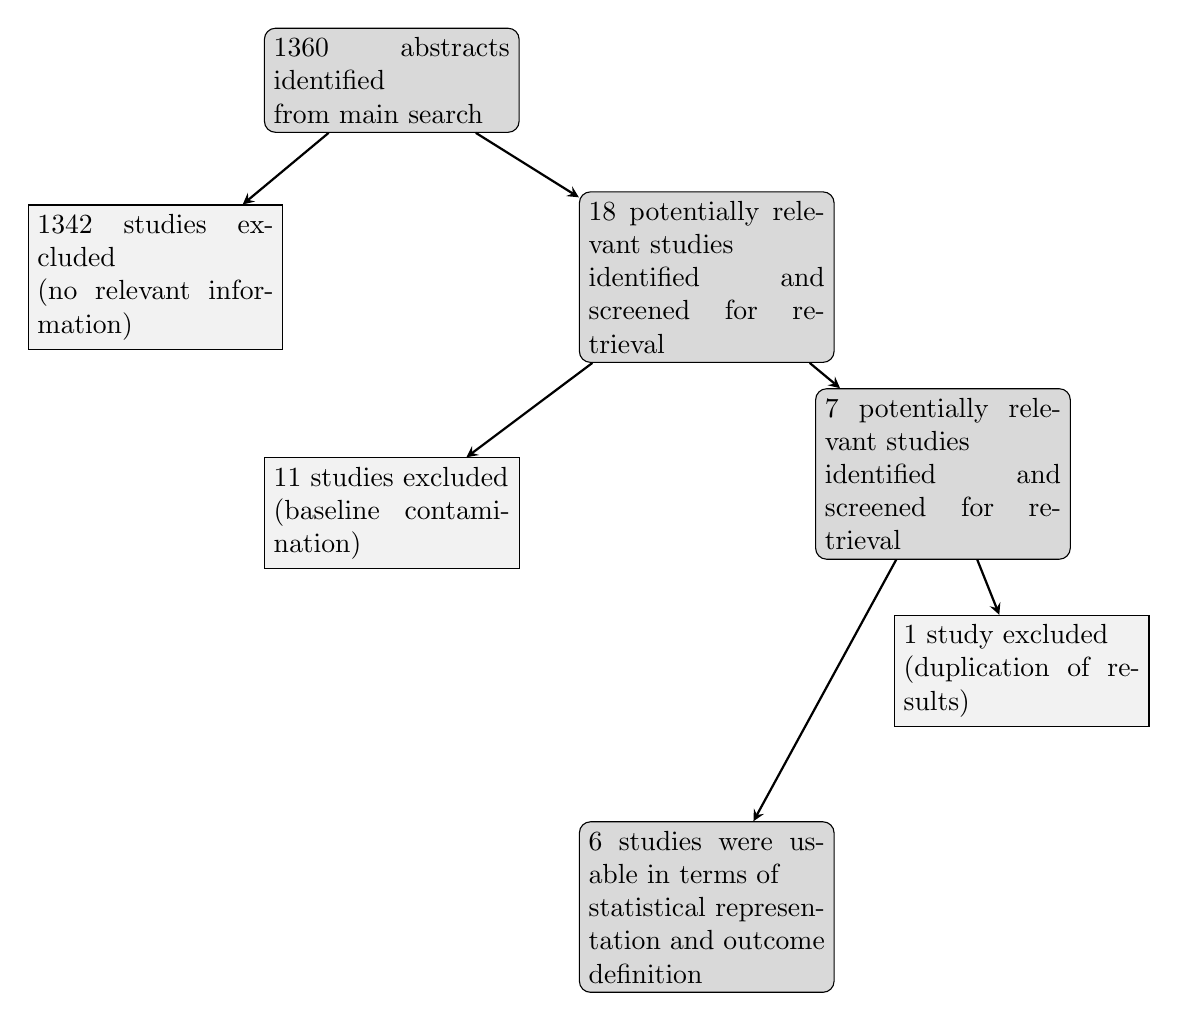
\begin{tikzpicture}[node distance=2cm]
        
        \node (start) [startstop] {\parbox{3cm}{1360 abstracts identified \\ from main search}};
        \node (exclude1) [process, below of=start, yshift=-0.5cm, xshift=-3cm] {\parbox{3cm}{1342 studies excluded \\ (no relevant information)}};
        \node (relevant1) [startstop, right of=exclude1, xshift=5cm] {\parbox{3cm}{18 potentially relevant studies \\ identified and screened for retrieval}};
        \node (exclude2) [process, below of=relevant1, yshift=-1cm, xshift=-4cm] {\parbox{3cm}{11 studies excluded \\ (baseline contamination)}};
        \node (relevant2) [startstop, right of=exclude2, xshift=5cm, yshift=0.5cm] {\parbox{3cm}{7 potentially relevant studies \\ identified and screened for retrieval}};
        \node (exclude3) [process, below of=relevant2, xshift=1cm, yshift=-0.5cm] {\parbox{3cm}{1 study excluded \\ (duplication of results)}};
        \node (usable) [startstop, below of=exclude3, yshift=-1cm, xshift=-4cm] {\parbox{3cm}{6 studies were usable in terms of \\ statistical representation and outcome definition}};
        
        % Arrows
        \draw [arrow] (start) -- (exclude1);
        \draw [arrow] (start) -- (relevant1);
        \draw [arrow] (relevant1) -- (exclude2);
        \draw [arrow] (relevant1) -- (relevant2);
        \draw [arrow] (relevant2) -- (exclude3);
        \draw [arrow] (relevant2) -- (usable);
        
        \end{tikzpicture}
    \end{figure}
    

\section{Statistical Analysis}

Statistical heterogeneity among studies was examined using both the Cochrane Q and the I\textsuperscript{2} statistics. For the Q statistic, a p-value of <0.10 was considered to be representative of statistically significant heterogeneity. I\textsuperscript{2} represents the percentage of total variation contributed by between-study variation. It ranges between 0\% and 100\%, and values of 25\%, 50\%, and 75\% were considered to represent low, moderate, and high heterogeneity, respectively (Higgins \& Thompson, 2002). A funnel plot with pseudo 95\% CIs was used for a visual assessment of publication bias. To test for publication bias, we used the STATA command metabias, which performs the Egger’s regression asymmetry test (Egger et al., 1997) and the Begg-adjusted rank correlation test (Begg \& Mazumdar, 1994). A p-value of <0.10 was considered to be representative of statistically significant publication bias. All statistical analyses were completed using STATA Version 10.1.

\section{Pathways}

In addition to the formal meta-analysis that aimed to quantify the dose–response relationship between alcohol consumption and the risk of unprovoked seizures and epilepsy, we examined the pathologic etiology of such relationships, in particular, biologic pathways, reversibility following interventions, temporality and consistency of the association, and relevant experimental studies.

\section{Results}

The meta-analysis of the studies (Ogunniyi et al., 1987; Ng et al., 1988; Leone et al., 1994, 1997, 2002; Zeng et al., 2003) on the risk of epilepsy given alcohol consumption resulted in a pooled RR of 2.19 (95\% CI 1.83–2.63) across all studies (Fig. 2). There was no significant heterogeneity between the studies (Q-test = 8.78, d.f. = 8 p = 0.361; I\textsuperscript{2} = 9\%, 95\% CI = 0–68\%). Visual inspections of the funnel plot (Fig. S1) and both the Egger’s (p = 0.754) and Begg’s tests (p = 0.417) revealed no significant asymmetry. These results suggest no evidence of substantial publication bias.

Several studies (Ng et al., 1988; Leone et al., 1994, 1997, 2002) provided data that allowed us to examine the dose–response relationship between the different levels of regular alcohol consumption and onset of epilepsy. The best fitting model can be seen in Fig. 3. Model fit statistics also indicated that it provided a good fit to the data (Q = 16.56, d.f. = 22, p = 0.787; I\textsuperscript{2} = 0\%, 95\% CI = 0–45\%). Up to the point of about 24 g of alcohol per day the curve between alcohol and the risk of epilepsy was relatively flat, after which, however, the risk curve increased steeply with increasing levels of consumption. Individuals consuming 12, 48, 72, and 96 g of alcohol daily had RRs of 1.17 (95\% CI = 1.13–1.21), 1.81 (95\% CI = 1.59–2.07), 2.44 (95\% CI = 2.00–2.97), and 3.27 (95\% CI = 2.52–4.26), respectively, relative to abstainers.

Studies by Leone et al. (1994, 1997, 2002) found that a high proportion of people with epileptic seizures were also alcohol dependent. This led us to the question of whether only heavy drinking was related to this problem, that is, does the relationship between alcohol consumption and epilepsy have a threshold? To test this relationship, a categorical meta-analysis was conducted including only studies that had data points for <50 g daily average consumption of pure alcohol (about four drinks). This meta-analysis included four studies, comprising seven independent datasets (Ng et al., 1988; Leone et al., 1994, 1997, 2002).



\begin{figure}[H]
    \centering
    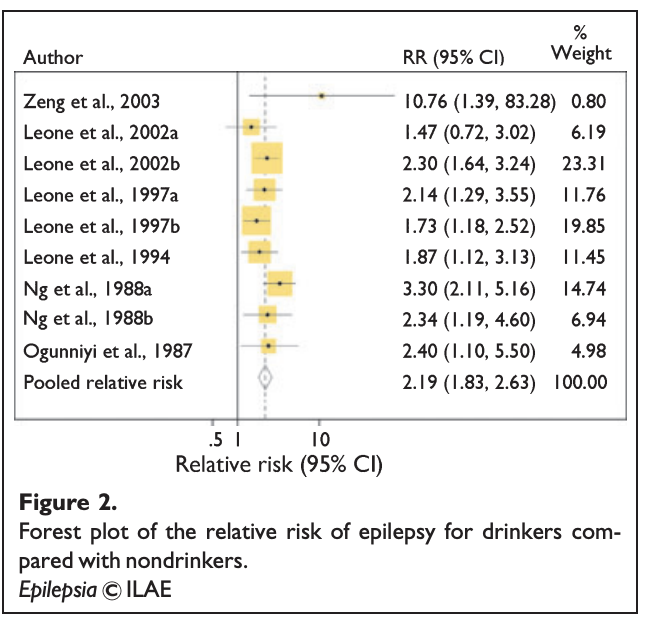
\includegraphics[width=\textwidth]{images/Screenshot 2024-10-22 at 10.11.42.png}
    \caption{Forest plot of the association between alcohol consumption and the risk of epilepsy.}
    \label{fig:forest_plot}
\end{figure}

\begin{figure}[H]
    \centering
    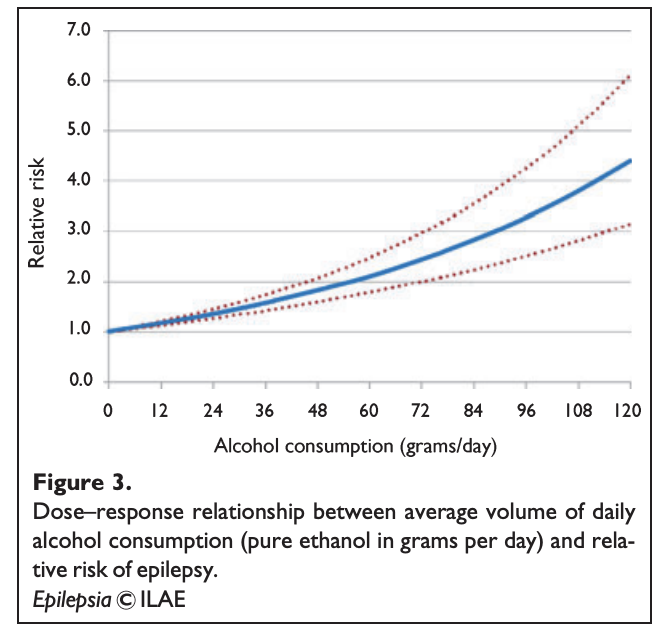
\includegraphics[width=\textwidth]{images/Screenshot 2024-10-22 at 10.12.52.png}
    \caption{Funnel plot with pseudo 95\% CIs for visual assessment of publication bias.}
    \label{fig:funnel_plot}
\end{figure}

\begin{figure}[H]
    \centering
    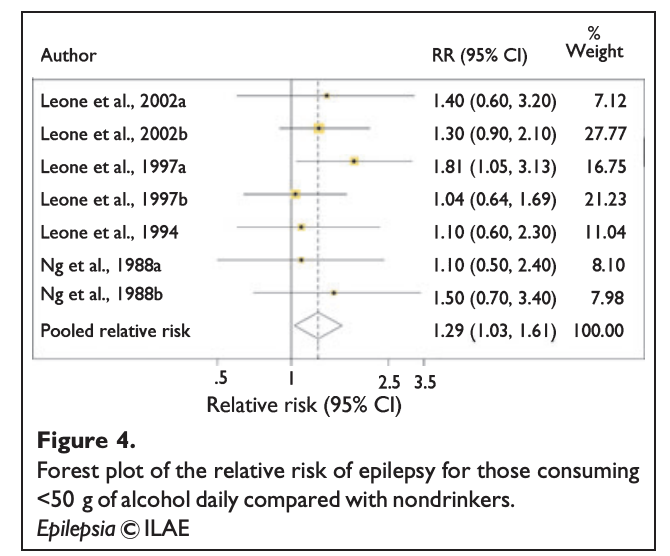
\includegraphics[width=\textwidth]{images/Screenshot 2024-10-22 at 10.13.21.png}
    \caption{Dose-response relationship between different levels of regular alcohol consumption and the risk of epilepsy.}
    \label{fig:dose_response}
\end{figure}


et al., 1988; Leone et al., 1994, 1997, 2002). There was no
evidence for the presence of heterogeneity between the
studies (Q = 2.79, d.f. = 6 p = 0.835; I\textsuperscript{2} = 0\%, 95\% CI =
0–71\%). The summary RR for consumption below 50 g of
alcohol daily was 1.29 (95\% CI = 1.03, 1.61) for all studies
combined (see Fig. 4).
Aggregated over all studies, the results indicated a
slightly elevated risk in comparison to abstainers, which
was barely significant (lower bound 1.03). A problematic
aspect of this result was that the comparison group comprised current abstainers. Consequently, it might be the case
that the slightly elevated risk was due to the sick quitter
effect, that is, people quitting drinking because of health
reasons (Shaper et al., 1988).

\section{Discussion}

\textbf{Study limitations}
The majority of published studies included, or were
restricted to, withdrawal seizures and only few studies were
dedicated solely to epileptic events. Several studies that we
included in the meta-analysis did not have clearly defined
outcomes. Ng et al. (1988), for example, reported on several
types of seizures, including withdrawal seizures. In order to
exclude the latter we included the data subset for unprovoked seizures, which according to the authors included idiopathic and remote symptomatic seizures. This was the
same approach that we used for categories of unprovoked
and idiopathic seizures when extracting data from the studies of Leone et al. (1994, 1997, 2002). Despite our best
attempts to extract the relevant data on nonwithdrawal seizures, some data on alcohol-withdrawal seizures may still
have been included in the meta-analysis. This might well
have affected the definitional clarity of the meta-analysis.
Therefore, further clinical research is required to make causal conclusions more clear and definitive.

\textbf{Heterogeneity of studies}
Studies that were included into meta-analysis used different outcomes, which could be divided into two categories—epilepsy and first-time seizures. We acknowledge that
combining such outcomes may be questionable; however,
we used the data on unprovoked seizures with the assumption that if a seizure occurs without an immediate cause
there should be a brain pathology that predisposes for a
recurrence of seizures. According to the newest definition
of epilepsy by ILAE and IBE (Fisher et al., 2005), one seizure and presence of predisposing factor, that is, occurrence
of one seizure may be considered an onset of epilepsy in certain cases. Although this definition is still a subject of discussion in the scientific literature, current evidence shows
that the probability of recurrence of seizures in persons who
had one seizure is high (Fisher \& Lepik, 2008).

\textit{Association and strength of association}
The meta-analysis of existing case–control studies
revealed a clear association between alcohol consumption
and the risk of onset of epilepsy or seizures. Heterogeneity
of studies reflecting the relationship between alcohol consumption and onset of seizures or epilepsy in various settings is the evidence of consistency of this association.

\textit{Biologic gradient and threshold testing}
The existence of a threshold relationship between alcohol
consumption and the risk of epilepsy remains undetermined.
However, we found evidence of a clear dose–response relationship as is reflected in Fig. 3. Based on the statistical part
of the research we can clearly state that alcohol consumption is a predisposing factor for epilepsy and single seizures.
However, further clinical research is needed before a more


\textit{assertive conclusion}
An assertive conclusion can be made about the causal relationship between alcohol consumption and the onset of epilepsy as an independent disease.

\textit{Temporality}
According to clinical observations, repetitive unprovoked seizures appear after 10 or more years of heavy alcohol consumption (Devetag et al., 1983). A multiple-stage model of epilepsy related to chronic alcohol consumption proposed by Bartolomei fits this timeline (Bartolomei, 2006). However, this theory is based primarily on the ‘‘kindling’’ hypothesis, which cannot be considered a unique biologic pathway of development of epilepsy in chronic alcohol abusers.

\textit{Plausibility and coherence}
Chronic alcohol consumption has diverse effects on the central nervous system, affecting its structure and functioning in several ways. There are theories explaining epileptogenesis in alcohol users including brain traumas, hypoxia, and kindling; each is briefly described below. Dam and colleagues observed that 74% of long-term heavy alcohol users with epilepsy had cerebral atrophy as a consequence of chronic alcohol intake. Positioning cerebral atrophy as a precipitating factor for the onset of epilepsy allowed them to connect it as a causal link between alcohol consumption and epilepsy (Dam et al., 1985). However, a comparative study of alcoholic patients (with at least a 3-year history of alcoholism, 8 years on average) with and without epilepsy revealed similar rates of cerebral atrophy in both groups, albeit the cerebral atrophy in alcohol users with epilepsy was more generalized. This led the authors to the conclusion that more generalized forms of cerebral atrophy may cause epilepsy in alcohol users (Meyer-Wahl & Braun, 1982). Other structural changes such as cerebrovascular infarctions, lesions, and head traumas have been found to be more prevalent in heavy alcohol users and people with alcohol dependence and have been reported to be a direct cause of repetitive epileptic seizures in multiple studies (Dam et al., 1985; Rathlev et al., 2006).

A ‘‘kindling’’ theory proposed by Ballenger and Post states that repeated withdrawal, including natural withdrawal through sleep over the years, leads to the gradual lowering of the epileptogenic threshold (Ballenger \& Post, 1978). Although this theory is the most plausible explanation of ethanol effects on the central nervous system (CNS), it does not include other factors described previously, which in turn cannot be completely excluded for analysis.

The occurrence of seizures in alcohol users can also be explained by certain changes in neurotransmitter systems and metabolism (ionic imbalance and hypoglycemia) that cause hyperexcitability. One of the most important of these changes is under-regulation of the expression of c-aminobutyric acid (GABA)A receptors, in which a reduction in the sensitivity of GABA receptors corresponds to a decrease of inhibitory action-related GABA (Frye \& Fincher, 1988).

\textit{Reversibility following treatment}
A systematic search for clinical trials demonstrating
improvements of epilepsy symptoms in alcohol users
through treatment did not result in any studies supporting
the reversibility of epilepsy.

\textit{Experimental evidence}
For ethical reasons, experimental evidence on alcohol-induced seizures and epilepsy is limited to animal studies.
In particular, repeated withdrawals were associated with the
onset of spontaneous seizures, and correlated with the duration and quantity of withdrawals and a lowering of the convulsive threshold in rats (Kokka et al., 1993). In addition,
Scorza and coauthors showed that alcohol withdrawal was a
crucial event for the development of functional and neuropathologic alterations associated with epilepsy (Scorza
et al., 2003). Although the animal studies are informative in
terms of alcohol-related epileptogenesis, the findings cannot
be easily extrapolated to humans.

In summary, the current evidence shows a strong and consistent association between alcohol consumption and epilepsy or unprovoked seizures, although this association and
its strength may be refined in further research, which may
also include the identification of a threshold. The existing
research allowed us to calculate the dose–response relationship for the amount of alcohol regularly consumed and the
risk of developing epilepsy or unprovoked seizures in
chronic alcohol users. Several pathogenic mechanisms for
the development of epilepsy in heavy drinkers were

\section{Conclusions}
The dose–response relationship between alcohol consumption and epilepsy and unprovoked seizures was quantified and several pathogenic mechanisms were suggested, although none of them has been shown to be the unique causative pathway for epilepsy. Certain limitations underlying this study require further research to clarify the outstanding statistical issues and pathogenesis of epilepsy in heavy drinkers.

\section{Acknowledgments}
This work was financially supported by contract \# HHSN267200700041C from NIAAA ‘‘Alcohol- and Drug-Attributable Burden of Disease and Injury in the US’’ and a small contribution of the Global Burden of Disease (GBD) Study to the last author. We would like to thank Robin Room, Theo Vos, and the core group of the Comparative Risk Assessment within the GBD 2005 Study for alcohol for support and comments on the general methodology and an earlier version of this article. In addition, we would like to thank Fotis Kanteres for editing this article. We confirm that we have read the Journal’s position on issues involved in ethical publication and affirm that this report is consistent with those guidelines.

\section{Disclosure}
None of the authors has any conflict of interest to disclose.


\section{References}
Alldredge BK, Lowenstein DH. (1993) Status epilepticus related to alcohol abuse. Epilepsia 34:1033–1037.

Ballenger JC, Post RM. (1978) Kindling as a model for alcohol withdrawal syndromes. Br J Psychiatry 133:1–14.

Barclay GA, Barbour J, Stewart S, Day CP, Gilvarry E. (2008) Adverse physical effects of alcohol misuse. Advances in Psychiatric Treatment 14:139–151.

Bartolomei F. (2006) Epilepsy and alcohol. Epileptic Disord 8:S72–S78.

Begg CB, Mazumdar M. (1994) Operating characteristics of a rank correlation test for publication bias. Biometrics 50:1088–1101.

Bell GS, Sander JW. (2001) The epidemiology of epilepsy: the size of the problem. Seizure 10:306–314.

Brennan FN, Lyttle JA. (1987) Alcohol and seizures: a review. J R Soc Med 80:571–573.

Dam AM, Fuglsang-Frederiksen A, Svarre-Olsen U, Dam M. (1985) Late-onset epilepsy: etiologies, types of seizure, and value of clinical investigation, EEG, and computerized tomography scan. Epilepsia 26:227–231.

DerSimonian R, Laird N. (1986) Meta-analysis in clinical trials. Control Clin Trials 7:177–188.

Devetag F, Mandich G, Zaiotti G, Toffolo GG. (1983) Alcoholic epilepsy: review of series and proposed classification and etiopathogenesis. Ital J Neurol Sci 4:275–284.

Egger M, Smith GD, Schneider M, Minder C. (1997) Bias in meta-analysis detected by a simple, graphical test. BMJ 315:629–634.

English D, Holman C, Milne E, Winter M, Hulse G, Codde G, Bower G, Corti B, de Klerk N, Knuiman M, Kurinczuk J, Lewin G, Ryan G. (1995) The quantification of drug caused morbidity and mortality in Australia 1995. Commonwealth Department of Human Services and Health, Canberra, Australia.

Ezzati M, Lopez AD, Rodgers AD, Vander Horn S, Murray CJL, Comparative Risk Assessment Collaborating Group. (2002) Selected major risk factors and global and regional burden of disease. Lancet 360:1347–1360.

Fernandes PT, Salgado PCB, Noronha ALA, Barbosa FD, Souza EAP, Li LM. (2004) Stigma scale of epilepsy: conceptual issues. J Epilepsy Clin Neurophysiol 10:213–218.

Fisher RS, van Emde Boas W, Blume W, Elger C, Genton P, Lee P, Engel J. (2005) Epileptic seizures and epilepsy: definitions proposed by the international league against epilepsy (ILAE) and the international bureau for epilepsy (IBE). Epilepsia 46:470–472.

Fisher RS, Lepik I. (2008) Debate: When does a seizure imply epilepsy? Epilepsia 49:7–12.

Frye GD, Fincher AS. (1988) Effect of ethanol on gamma-vinyl GABA-induced GABA accumulation in the substantia nigra and on synaptosomal GABA content in six rat brain regions. Brain Res 449:71–79.

Greenland S, Longnecker MP. (1992) Methods for trend estimation from summarized dose-response data, with applications to meta-analysis. Am J Epidemiol 135:1301–1309.

Higgins JP, Thompson SG. (2002) Quantifying heterogeneity in a meta-analysis. Stat Med 21:1539–1558.

Higgins JP, Thompson SG, Deeks JJ, Altman DG. (2003) Measuring inconsistency in meta-analyses. BMJ 327:557–560.

Hillbom M, Pieninkeroinen I, Leone M. (2003) Seizures in alcohol-dependent patients. CNS Drugs 17:1013–1030.

Jacoby A. (2002) Stigma, epilepsy, and quality of life. Epilepsy Behav 3:10–20.

Jallon P. (2002) Epilepsy and epileptic disorders, an epidemiological marker? Contributions of descriptive epidemiology. Epileptic Disord 4:1–13.

Kokka N, Sapp DW, Taylor AM, Olsen RW. (1993) The kindling model of alcohol dependence: similar persistent reduction in seizure threshold to pentylenetetrazol in animals receiving chronic ethanol or chronic pentylenetetrazol. Alcohol Clin Exp Res 17:525–531.

Leonardi M, Ustun TB. (2002) The global burden of epilepsy. Epilepsia 43:21–25.

Leone M, Bottacchi E, Gionco M, Nardozza V, Sironi L. (1994) Alcohol and epileptic seizures: a case control study. Alcologia 6:215–219.

Leone M, Bottachi E, Beghi E, Morgando E, Mutani R, Amedeo G, Cremo R, Gianelli M, Ravagli Ceroni L. (1997) Alcohol use is a risk factor for a first generalized tonic-clonic seizure. Neurology 48:614–620.

Leone M, Bottacchi E, Beghi E, Morgando E, Mutani R, Cremo R, Ravagli Ceroni L, Floriani I. (2002) Risk factors for a first generalized tonic-clonic seizure in adult life. Neurol Sci 23:99–106.

Meyer-Wahl JG, Braun J. (1982) Epileptic seizures and cerebral atrophy in alcoholics. J Neurol 228:17–32.

Ng SKC, Hauser AW, Brust JCM, Susser M. (1988) Alcohol consumption and withdrawal in new-onset seizures. N Engl J Med 319:666–673.

Ogunniyi A, Osuntokun BO, Bademosi O, Adeuja AOG, Schoenberg BS. (1987) Risk factors for epilepsy: case-control study in Nigerians. Epilepsia 28:280–285.

Orsini NBR, Greenland S. (2006) Generalized least squares for trend estimation of summarized dose-response data. Stata J 6:40–57.

Rathlev NK, Ulrich AS, Delanty N, D’Onofrio G. (2006) Alcohol-related seizures. J Emerg Med 31:157–163.

Rehm J, Room R, Monteiro M, Gmel G, Graham K, Rehn N, Sempos C, Jernigan D. (2003) Alcohol as a risk factor for global burden of disease. Eur Addict Res 9:157–164.

Royston P, Sauerbrei W. (2008) Multivariable model-building: a pragmatic approach to regression analysis based on fractional polynomials for modelling continuous variables. John Wiley \& Sons, Hoboken, NJ.

Scorza FA, Arida RM, Cysneiros RM, Priel MR, de Albuquerque M, Cavalheiro EA. (2003) The effects of alcohol intake and withdrawal on the seizures frequency and hippocampal morphology in rats with epilepsy. Neurosci Res 47:323–328.

Shaper A, Wannamethee G, Walker M. (1988) Alcohol and mortality in British men: explaining the U-shaped curve. Lancet 2:1267–1273.

Tsai G, Coyle JT. (1998) The role of glutamatergic neurotransmission in the pathophysiology of alcoholism. Annu Rev Med 49:173–184.

Zeng J, Zhen H, Mao-Sheng H, Mei-Hua J. (2003) A case-control study on the risk factors and other socio-psychological factors of epilepsy. Chin J Epidemiol 24:116–118.

\section*{Supporting Information}
Additional Supporting Information may be found in the
online version of this article:
\begin{itemize}
    \item Figure S1. Begg’s funnel plot. Ln RR, natural logarithm
    of relative risk; SE, standard error.
\end{itemize}
Please note: Wiley-Blackwell is not responsible for the
content or functionality of any supporting information supplied by the authors. Any queries (other than missing material) should be directed to the corresponding author for the
article.


\end{document}
